\documentclass{article}

\usepackage[preprint]{neurips_2026}
\usepackage[T1]{fontenc}
\usepackage[utf8]{inputenc}
\usepackage{microtype}
\usepackage{url}
\usepackage{booktabs}
\usepackage{graphicx}
\usepackage{amsmath}

\title{Phase-Aware Pooled Rideshare Dispatch on a Real London Map}

\author{%
  Ahmad Alashoury \\
  \And
  Koroush Emari \\
  \And
  Abdelrahman El Banna \\
  \And
  Shikar Srivastava
}

\begin{document}

\maketitle

\begin{abstract}
We study reinforcement learning for pooled rideshare dispatch on a real OpenStreetMap extract of downtown London, Ontario. The problem is intentionally harder than a toy pickup-and-dropoff benchmark: one vehicle with two seats must serve four riders while reasoning about traffic phases, deadlines, and pooling quality. Our main technical contribution is a \emph{phase-aware, hub-level dispatch formulation} that separates high-level stop selection from low-level path following. Instead of learning to drive cell by cell, the agent chooses the next pickup or dropoff stop and the environment executes the shortest path on the real street graph. We combine this abstraction with legal-action masking and curriculum training, then compare Q-learning, SARSA, DQN, and PPO. Over three random seeds, all four methods achieve full task completion, but DQN produces the best service quality: 58.3\% on-time riders, 1.67 late dropoffs on average, and 43.4 steps per episode. The results suggest that compact real-map dispatch environments can be learned by standard RL methods, but neural value approximation is better than tabular methods at exploiting recurring traffic- and rider-pattern structure.
\end{abstract}

\section{Introduction}
Urban rideshare systems must make decisions under uncertainty: which rider should be picked up first, when should the platform pool riders together, and how should congestion affect the route order? The core challenge is not only path finding. It is a sequential service problem in which local decisions can make later riders late, reduce pooling efficiency, or force expensive detours.

This project studies that decision problem as a reinforcement learning (RL) task. The setting is a single Uber-style vehicle operating on a real downtown London, Ontario street graph derived from OpenStreetMap. The vehicle has two seats and must serve four riders. Each rider has a pickup hub, a dropoff hub, and a delivery-style deadline. The environment also includes traffic phases representing commute, event, and nightlife congestion.

The problem is difficult for existing techniques for three reasons. First, exact dynamic assignment methods can optimize a given batch of trips, but they typically require hand-crafted objectives, known demand, or repeated re-solving and do not naturally learn reusable dispatch policies \citep{alonso2017ride}. Second, tabular RL methods suffer from rapid state growth once multiple riders, deadlines, and traffic contexts are included \citep{watkins1992q, rummery1994line}. Third, end-to-end low-level control wastes learning capacity on movement mechanics when the research question is really about dispatch order.

Our intuition is that the rideshare problem becomes both realistic and learnable if we factor it into two layers. The environment should handle shortest-path routing on a real map, while RL should learn the \emph{next stop selection policy}. We implement this idea as a phase-aware, hub-level Markov decision process (MDP) with legal-action masking and curriculum training, then compare Q-learning, SARSA, DQN, and PPO under the same benchmark.

\section{Techniques To Tackle the Problem}

\subsection{Previous Work}
Classical RL baselines remain useful reference points for dispatch problems. Q-learning learns action values by bootstrapping toward the greedy next action \citep{watkins1992q}, while SARSA performs an on-policy update using the next action actually taken \citep{rummery1994line}. Deep Q-Networks (DQN) replace tabular value storage with a neural approximation and replay buffer, enabling generalization across related states \citep{mnih2015dqn}. PPO provides a stable policy-gradient baseline through clipped policy updates \citep{schulman2017ppo}.

Transportation and fleet-management work has shown that realistic dispatching and pooling create large, stochastic decision spaces. Alonso-Mora et al.\ formulate dynamic trip--vehicle assignment for high-capacity ride-sharing and show the value of explicit assignment optimization \citep{alonso2017ride}. Oda and Joe-Wong propose MOVI, a model-free DQN-based fleet management framework, highlighting that learned policies can outperform handcrafted dispatch baselines at scale \citep{oda2018movi}. Lin et al.\ extend this direction with contextual multi-agent deep RL for large-scale fleet management \citep{lin2018fleet}. These papers motivate our project, but they target large-fleet or centralized rebalancing settings rather than a compact, presentation-friendly benchmark where individual dispatch choices remain interpretable.

\subsection{Our Technique}
The main technique we developed is not a brand-new RL algorithm. Instead, it is a \textbf{new dispatch formulation} that makes a realistic rideshare problem tractable for standard RL baselines. It has four parts.

\paragraph{(1) Real-map, hub-level abstraction.}
We start from a real OpenStreetMap extract of downtown London. We rasterize the road network into a \(28 \times 28\) grid, keep the largest connected component, and anchor named hubs such as London Station, Covent Garden Market, Canada Life Place, London City Hall, Victoria Park, Museum London, Grand Theatre, Central Library, Fanshawe Downtown, and Armouries Hotel. The resulting benchmark contains 335 road cells, 10 hubs, and 3 start depots.

\paragraph{(2) Dispatch instead of driving.}
The agent does not choose north, south, east, or west. It chooses one of eight high-level actions: pickup rider \(1\ldots4\) or dropoff rider \(1\ldots4\). Once the agent chooses a stop, the environment executes the shortest path over the real road graph. This design focuses learning on stop ordering and service quality instead of low-level locomotion.

\paragraph{(3) Phase-aware congestion and clustered demand.}
Each episode activates one traffic phase: \emph{Commute Rush}, \emph{Event Surge}, or \emph{Nightlife Rush}. Phase-specific penalty zones are layered on top of the base hotspot roads. Rider demand is also phase-conditioned through three templates: \emph{Commute Wave}, \emph{Event Exit}, and \emph{Culture Loop}. This creates structured scenarios in which the same dispatch policy should adapt differently under different traffic and rider mixes.

\paragraph{(4) Legal-action masking with curriculum training.}
Illegal actions are masked: riders cannot be picked up when the car is full, and riders cannot be dropped off before pickup. We also use an easy-to-hard curriculum. Early in training, episodes use two riders, one phase, and larger deadline slack; later episodes use all four riders, all phases, and tighter deadlines. The goal is to teach basic dispatch structure before requiring full-service performance.

\subsection{Benchmark Construction Pipeline}
The benchmark is generated in four explicit stages. First, we parse a real OpenStreetMap export of downtown London and keep only drivable street segments. Second, we project those coordinates onto a \(28 \times 28\) lattice, rasterize road segments into grid cells, and retain the largest connected component to avoid disconnected fragments. Third, we snap named downtown landmarks to their nearest usable road cells and promote them to hubs or depots. Finally, we overlay benchmark-specific logic: traffic hotspots, phase-dependent congestion regions, clustered rider-demand templates, and deadline heuristics.

This pipeline matters because it explains where the realism comes from. The \emph{geometry} is real: hubs are placed on an actual downtown road skeleton. The \emph{decision problem} is custom: traffic phases, pooling bonuses, and demand templates are engineered to create recurring but nontrivial dispatch patterns. In other words, we are not claiming to simulate Uber exactly. We are building a realistic, reproducible RL benchmark whose structure can be inspected and justified.

\section{Problem Formulation}

\subsection{State}
For tabular methods, the symbolic state is
\[
s = (\text{position}, \text{phase}, \text{carrying count}, \text{request signature}),
\]
where each rider contributes a tuple containing pickup hub, dropoff hub, status, deadline bucket, and wait bucket. Rider status is one of \(\{\text{waiting}, \text{onboard}, \text{delivered}\}\).

For neural methods, we use a 187-dimensional feature vector. It includes one-hot current location over 11 mobility nodes, one-hot carrying count, one-hot traffic phase, per-action legality and normalized target-distance features, per-rider structured features, and global progress indicators such as delivered fraction, late-dropoff fraction, peak occupancy, and step fraction.

The dual representation is an engineering compromise. The compact symbolic state allows Q-learning and SARSA to remain feasible on a laptop, while the dense 187-dimensional observation gives DQN and PPO enough structure to exploit similarities across rider configurations. This is also part of the comparison logic: if the benchmark is truly structured, the neural methods should be able to use these richer features to generalize better than the tabular baselines.

\subsection{Actions}
There are eight actions:
\[
\{\text{pickup}_1,\dots,\text{pickup}_4,\text{dropoff}_1,\dots,\text{dropoff}_4\}.
\]
Action masking enforces simple domain rules. A pickup is legal only if the rider is still waiting and capacity is available. A dropoff is legal only if the rider is onboard.

\subsection{Transition Dynamics and Traffic}
After the agent selects a legal action, the environment computes the shortest path from the current mobility node to the action's target hub and executes that path cell by cell. Time advances on every traversed road cell. During that travel, each unfinished rider loses one unit of deadline budget; riders not yet picked up accumulate waiting time, while riders already onboard accumulate ride time. Once the vehicle reaches the target hub, the corresponding pickup or dropoff transition is applied.

Traffic is modeled as an additive phase-dependent traversal penalty rather than as a separate microscopic vehicle simulation. The map contains base hotspot roads inferred from frequent street usage during rasterization, and each episode activates one of three phase maps: \emph{Commute Rush}, \emph{Event Surge}, or \emph{Nightlife Rush}. These phases raise the cost of traveling near specific landmark clusters such as London Station, Canada Life Place, Grand Theatre, and Covent Garden Market. This choice keeps the state compact while still making dispatch order phase-sensitive.

\subsection{Deadlines, Waiting Time, and Scenario Generation}
Each rider is assigned a deadline budget at the start of the episode. The budget is computed from three pieces: distance from the depot to the rider's pickup, distance from pickup to dropoff, and an additional slack term controlled by the curriculum stage. This means deadlines are not arbitrary; they are tied to the actual geometry of the scenario. A rider is marked late only if the vehicle completes the dropoff after that deadline budget reaches zero.

Demand is generated from clustered templates rather than uniform random sampling. For example, an event-phase episode samples riders near event-related hubs with a bias toward realistic pickup/dropoff pairings. This choice increases the chance of meaningful pooling and makes the same dispatch policy behave differently under commute, event, and nightlife conditions. Without such structure, the environment would mostly test generic path-finding rather than rideshare reasoning.

\subsection{Reward}
The reward is shaped around service quality. For each road cell traversed, the environment applies:
\begin{itemize}
    \item travel cost: \(-0.18\),
    \item unfinished-workload penalty: \(-0.04 \times\) remaining undelivered riders,
    \item traffic penalty for the active phase,
    \item pooling bonus: \(+0.12 \times \max(0,\text{occupancy}-1)\).
\end{itemize}
Successful pickups receive \(+10\), with an extra \(+4\) if the vehicle reaches occupancy two. On-time dropoffs receive \(+28\), while late dropoffs receive \(+18\). Invalid actions are penalized by \(-8\), and timing out at the episode limit adds \(-12\). Finishing all riders gives \(+22\), with bonuses for zero late riders \((+10)\) and successful pooling \((+8)\).

The reward was designed to encode three priorities at once. First, service should complete successfully, hence the large dropoff and terminal rewards. Second, service should be timely, hence the difference between on-time and late dropoffs plus the ongoing deadline pressure. Third, the policy should behave like a pooled rideshare driver rather than a sequence of isolated taxi trips, hence the occupancy-based shaping term and final pooling bonus. A pure shortest-path objective would miss all three of these priorities.

\begin{figure}[t]
    \centering
    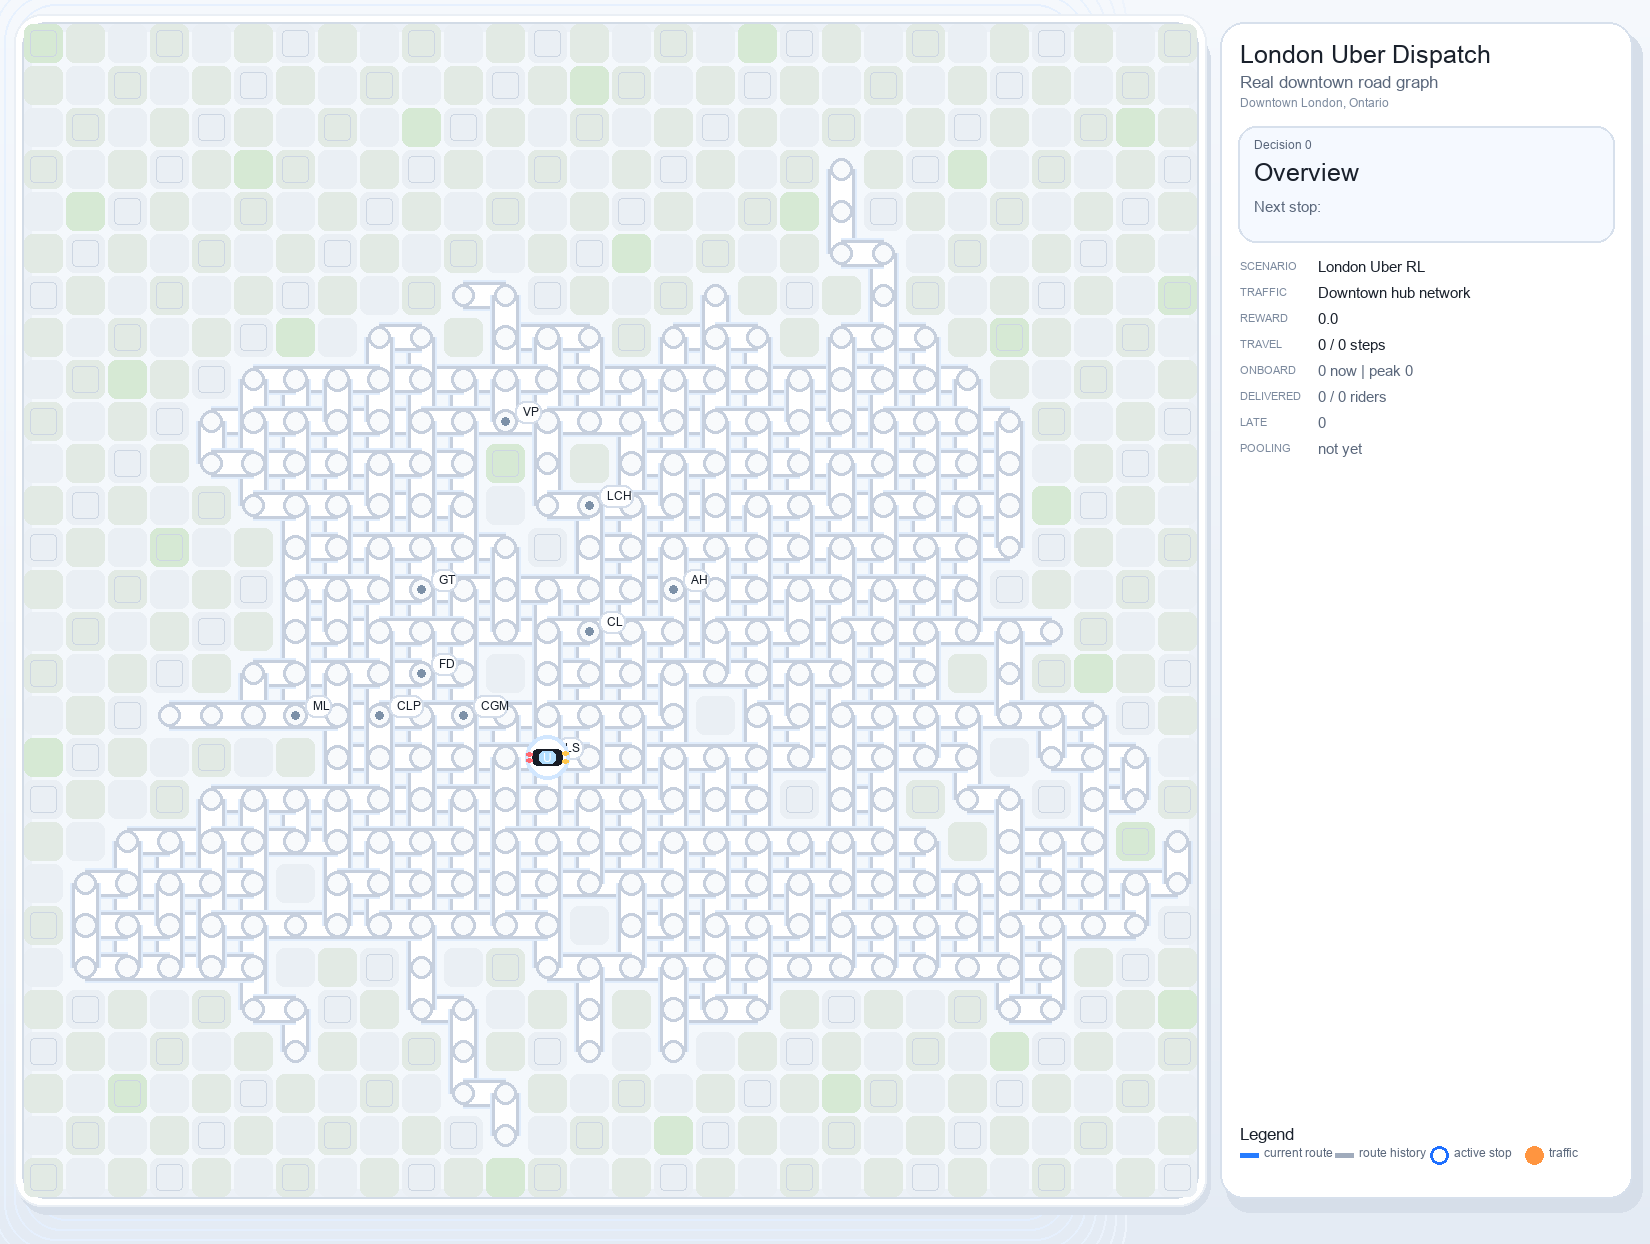
\includegraphics[width=0.48\linewidth]{map.png}\hfill
    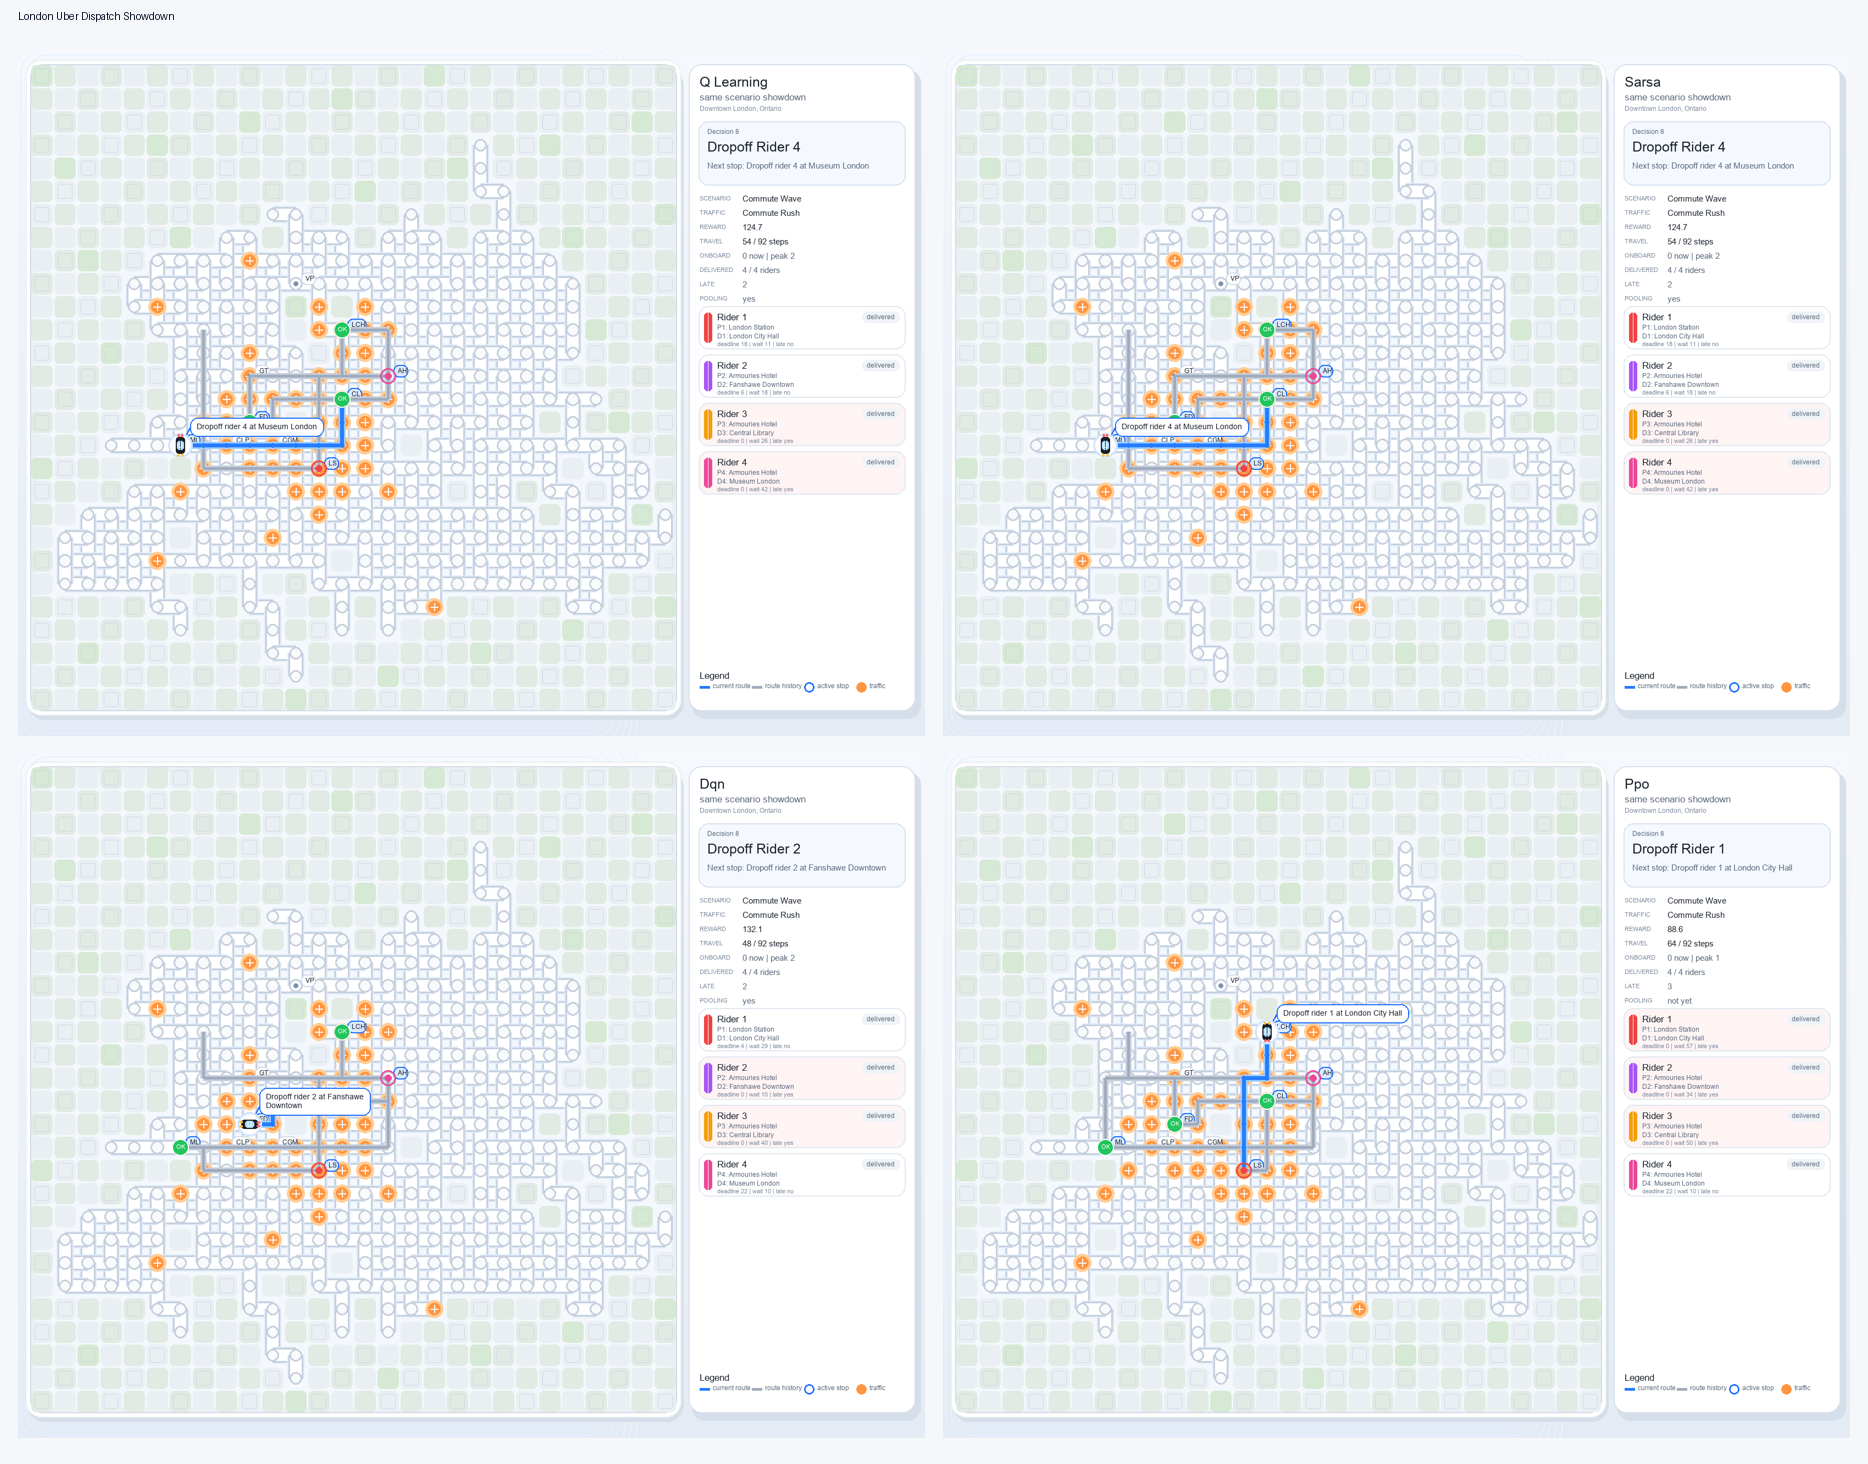
\includegraphics[width=0.48\linewidth]{showdown.png}
    \caption{Left: the processed London benchmark map. Right: a same-scenario qualitative comparison of the four learned policies.}
    \label{fig:map-showdown}
\end{figure}

\section{Evaluation}

\subsection{Experimental Setup}
We compare Q-learning, SARSA, DQN, and PPO. The current final report uses 3 random seeds, 900 training episodes per seed, and 20 greedy evaluation episodes per seed. We report mean reward, full-success rate, on-time rider rate, mean late dropoffs, pooling rate, peak occupancy, and mean evaluation steps.

The algorithm settings are intentionally comparable rather than heavily tuned. Q-learning uses learning rate 0.18 and discount 0.99; SARSA uses 0.14 and 0.985; DQN uses a 128-unit hidden layer, learning rate 0.0011, replay size 16{,}000, batch size 96, and target synchronization every 180 updates; PPO uses a 128-unit policy/value network, policy learning rate 0.001, value learning rate 0.002, 8 rollout episodes per update, and 8 optimization epochs.

We evaluate policies greedily so that the test-time metrics reflect the learned policy rather than exploration noise. The metrics are chosen to separate \emph{completion} from \emph{quality}. Full success rate measures whether all four riders are eventually served. On-time rider rate measures what fraction of served riders beat their deadlines. Late-dropoff count is the complementary penalty-focused metric. Pooling rate records whether the vehicle ever reached occupancy two, peak occupancy summarizes how aggressively the learned policy pooled riders, and step count measures route efficiency. This metric set matters because a benchmark in which all algorithms achieve 100\% completion can still reveal large practical quality differences.

\subsection{Baselines and Comparison Logic}
The four compared methods play different roles in the study. Q-learning is the classical off-policy tabular baseline; if it performs well, then the benchmark may still be simple enough for memorization. SARSA is the on-policy tabular counterpart and tests whether slightly more conservative value updates help in deadline-sensitive settings. DQN is the neural value-based baseline and is expected to benefit if the benchmark contains reusable structure across rider configurations and traffic phases. PPO is the policy-gradient baseline and is useful because it optimizes a stochastic policy directly rather than only learning action values.

This comparison setup lets us interpret outcomes rather than just rank methods. If tabular methods dominate, then our abstraction may still be too small. If PPO dominates, then policy learning may matter more than value approximation. If DQN dominates, then the likely story is that function approximation plus replay helps exploit repeated dispatch motifs. As shown below, the last pattern is what emerged in our experiments.

\subsection{Quantitative Results}
Table~\ref{tab:main-results} summarizes the main results. All four algorithms reach 100\% task completion on this benchmark, so completion itself is not the meaningful separator. The interesting differences appear in service quality.

\begin{table}[t]
    \centering
    \caption{Three-seed evaluation results on the London dispatch benchmark. Higher on-time rate is better; lower late dropoffs and steps are better.}
    \label{tab:main-results}
    \begin{tabular}{lcccc}
        \toprule
        Method & On-time (\%) & Late dropoffs & Pooling (\%) & Steps \\
        \midrule
        Q-learning & 53.3 & 1.87 & 100.0 & 45.55 \\
        SARSA & 52.1 & 1.92 & 100.0 & 45.78 \\
        DQN & \textbf{58.3} & \textbf{1.67} & 98.3 & \textbf{43.43} \\
        PPO & 56.7 & 1.73 & 93.3 & 45.43 \\
        \bottomrule
    \end{tabular}
\end{table}

\begin{figure}[t]
    \centering
    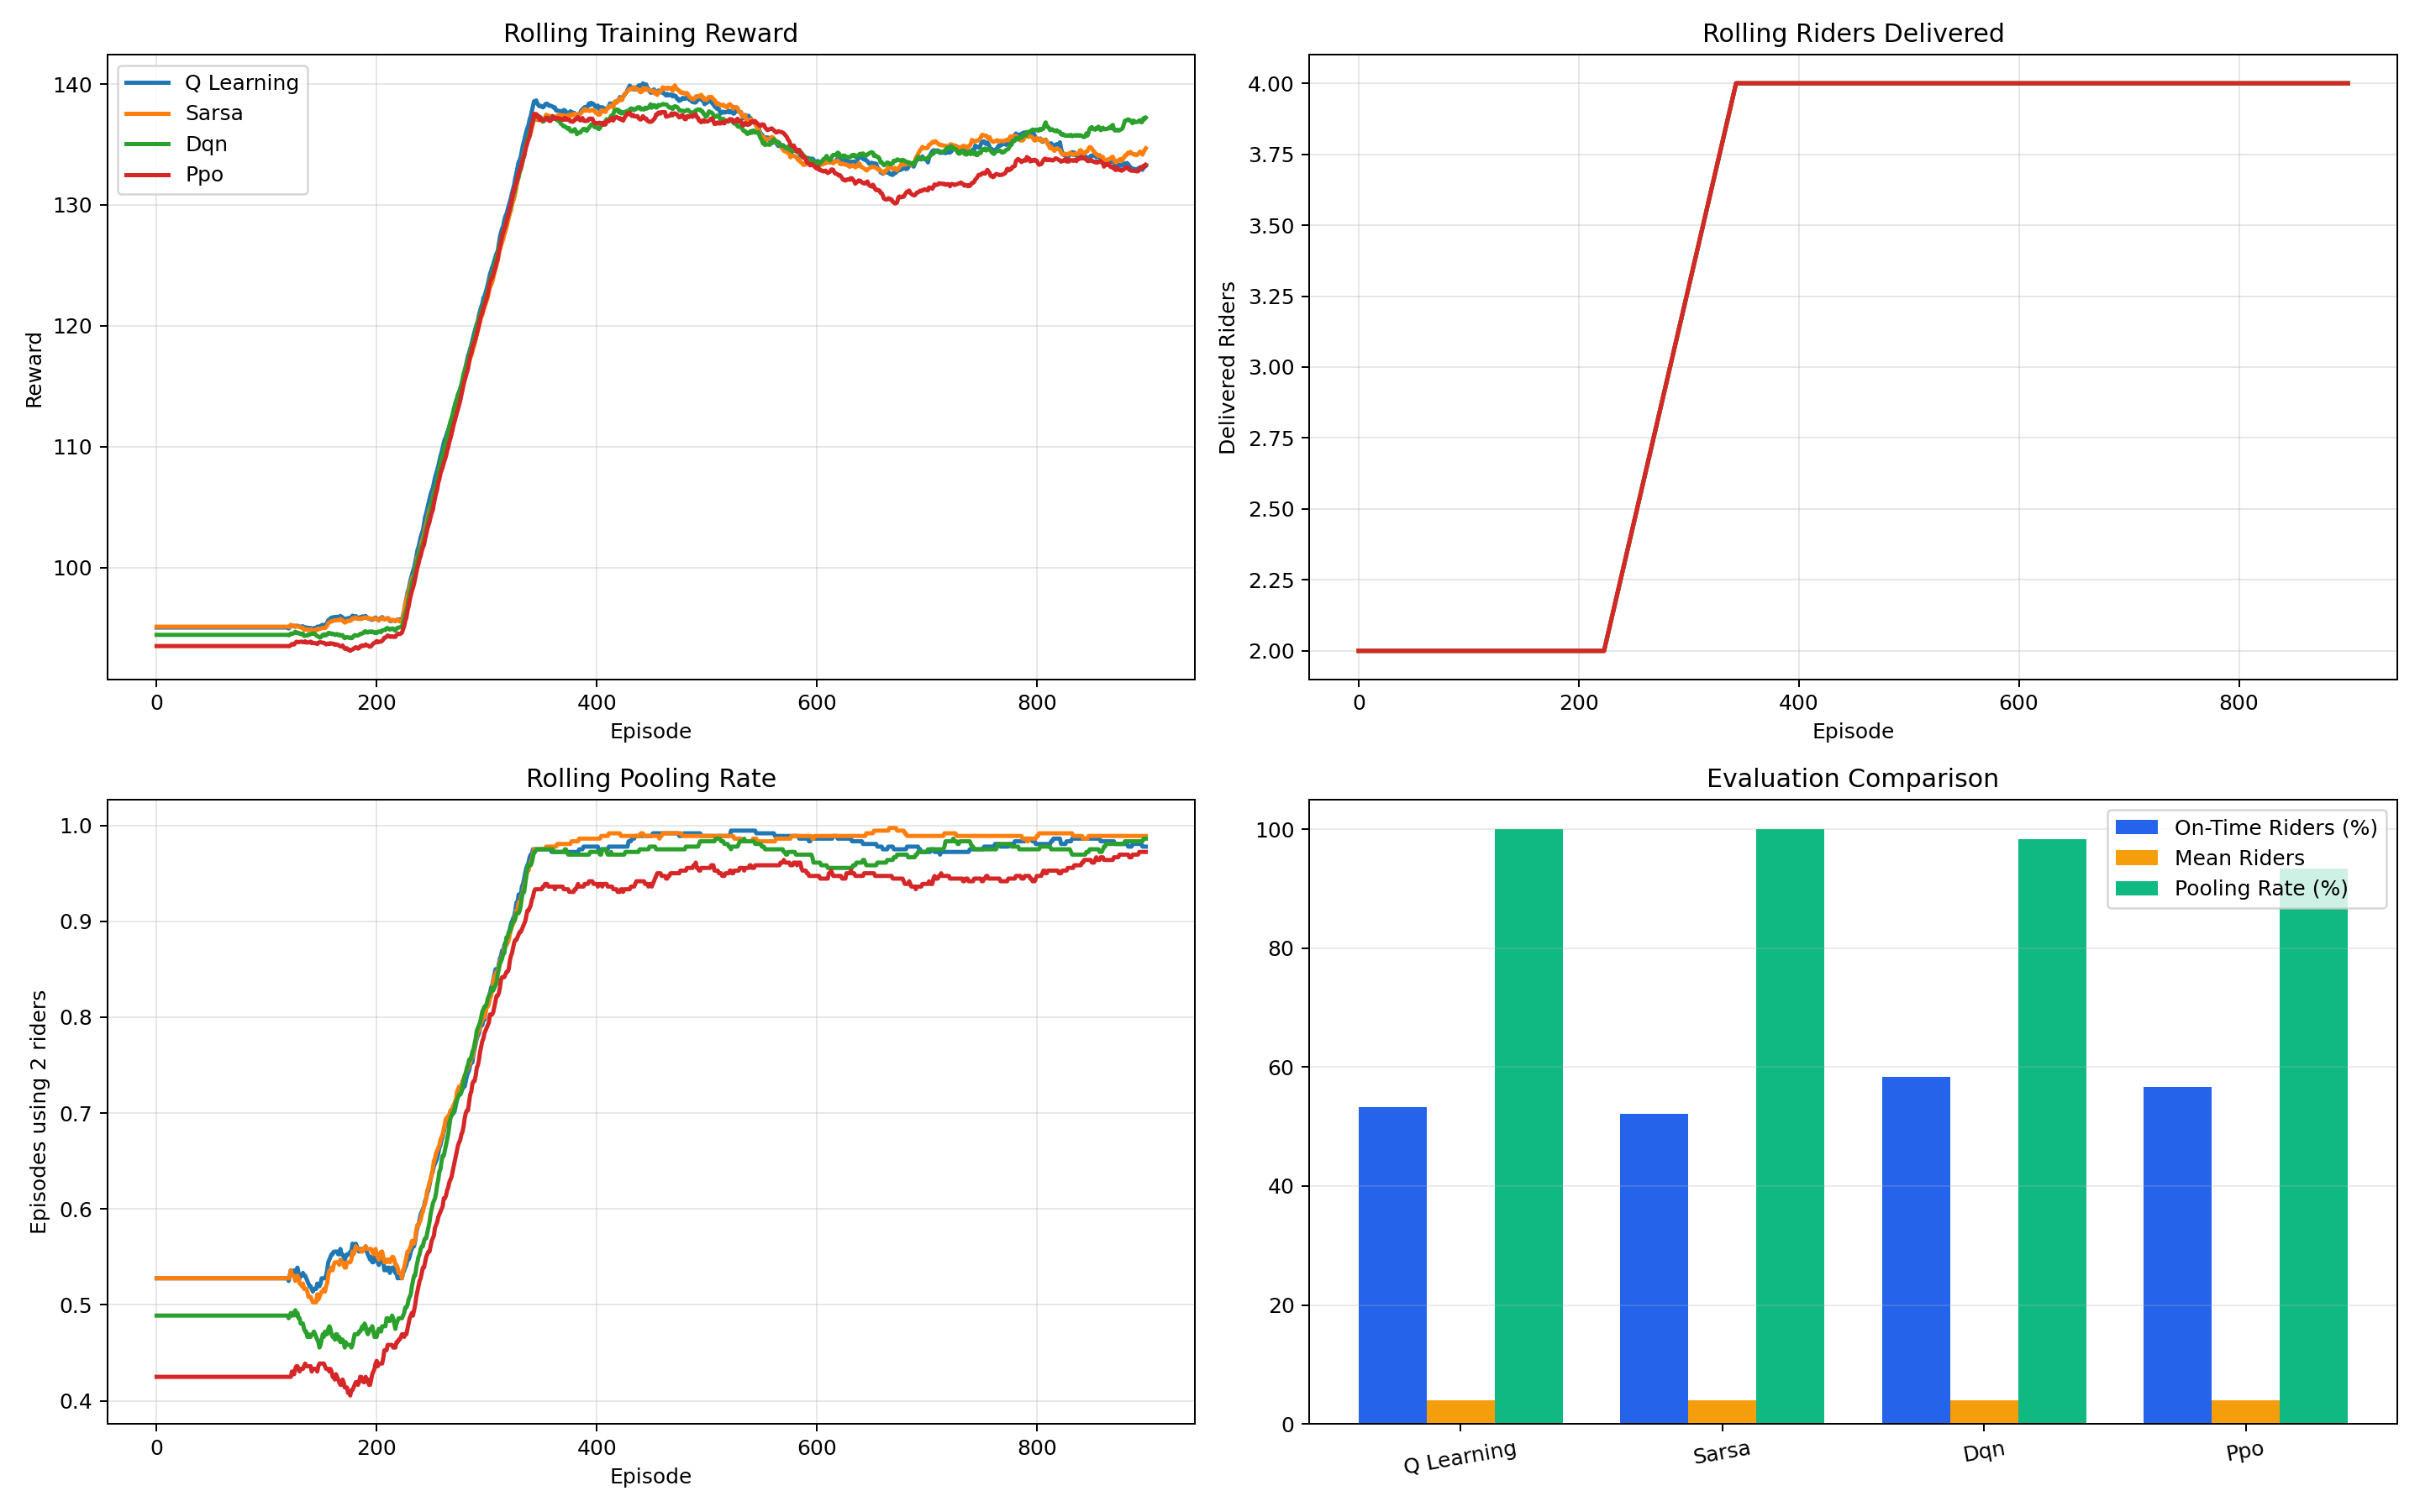
\includegraphics[width=\linewidth]{results_summary.png}
    \caption{Rolling training curves and aggregated evaluation results across the four algorithms.}
    \label{fig:summary}
\end{figure}

\subsection{Analysis}
The central empirical result is that DQN performs best overall. It achieves the highest on-time rider rate, the fewest late dropoffs, and the lowest evaluation step count. PPO is the closest competitor, but it pools slightly less consistently and uses more steps. Q-learning and SARSA solve the task but lag on timeliness.

This pattern matches the intuition behind our formulation. Once the problem includes multiple riders, deadlines, and phase-aware traffic, tabular state-action storage becomes less efficient. The symbolic state representation still expands quickly, and Q-learning/SARSA cannot generalize across nearby rider configurations. DQN can. PPO also generalizes, but in this benchmark it appears somewhat more sample-hungry than DQN.

The results also justify our design decision to evaluate more than task completion. If we reported only success rate, the methods would appear equivalent. The on-time rider rate and late-dropoff statistics reveal the actual quality gap.

\subsection{Qualitative Behavior}
The qualitative comparison in Figure~\ref{fig:map-showdown} reinforces the numerical results. DQN typically commits to more direct stop orderings once a phase-aware pattern has been recognized. PPO often finds similar routes but is somewhat less consistent about pooling two riders early in the episode. The tabular baselines can still solve the route set, but they more often choose service orders that create one or two extra detours, which then show up as higher step counts and more late riders.

This matters because the benchmark was designed to make such differences visible. Since the environment handles shortest-path travel automatically, any route inefficiency in the final visualization comes from the \emph{choice of next stop}, not from low-level navigation error. That is exactly the behavior we wanted to compare.

\subsection{Threats to Validity}
Our conclusions should be interpreted with a few limitations in mind. First, the benchmark uses a single vehicle and fixed rider batch per episode, so it is closer to compact pooled dispatch than to full marketplace simulation. Second, traffic is represented as additive road-cell penalties rather than dynamic travel-time uncertainty. Third, the present evaluation uses three seeds and moderate training budgets, which is enough to expose stable trends but not enough to claim fully tuned state-of-the-art performance.

\section{Conclusion}
We developed a phase-aware, action-masked pooled rideshare dispatch benchmark on a real OpenStreetMap extract of downtown London, Ontario. The key idea was to let the environment handle shortest-path routing while RL learns the next-stop dispatch policy. This makes the problem realistic enough to be interesting, but small enough to remain interpretable.

Our technique effectively tackles the problem in the sense that all methods learned viable policies and the benchmark exposes meaningful differences in service quality. Among the compared approaches, DQN performed best, indicating that neural value approximation is better suited than tabular baselines for this structured multi-rider setting.

Several limitations remain. The benchmark is single-vehicle, the traffic phase is fixed within an episode, and deadlines are deterministic. Future research should extend the environment to multi-vehicle coordination, online rider arrivals, stochastic congestion, fairness constraints, and richer hybrid approaches that combine offline demand models with online RL dispatch. A particularly promising direction is to compare learned dispatch against explicit assignment heuristics on exactly the same London benchmark, which would connect this compact academic environment back to the broader ride-sharing optimization literature.

\bibliographystyle{plainnat}
\bibliography{references}

\end{document}
